\documentclass[11pt]{article}
\usepackage[margin=1in]{geometry}
\usepackage{graphicx}
\usepackage{booktabs}
\usepackage{xcolor}
\usepackage{hyperref}
\usepackage{amsmath}
\usepackage{listings}
\usepackage{enumitem}
\usepackage{caption}
\usepackage{float}
\usepackage{longtable}
\usepackage{xurl}
\setlength{\emergencystretch}{3em}

\hypersetup{colorlinks=true, linkcolor=blue, urlcolor=blue, citecolor=blue}

\definecolor{codebg}{rgb}{0.96,0.96,0.96}
\lstset{
  basicstyle=\ttfamily\small,
  backgroundcolor=\color{codebg},
  frame=single,
  breaklines=true,
  columns=fullflexible,
  keywordstyle=\color{blue!70!black}\bfseries,
  commentstyle=\color{green!40!black}\itshape,
  stringstyle=\color{orange!70!black},
  language=C++,
  tabsize=2,
}
\lstdefinestyle{log}{language={}, basicstyle=\ttfamily\footnotesize, columns=fixed,
  keepspaces=true}

\title{\Large\textbf{Group Project Report: Address Resolution Protocol (ARP)\\
and Dynamic Host Configuration Protocol (DHCP)}}
\author{
\begin{tabular}{ll}
Rittick Dutta & 002410501088 \\
Saikat Nayek & 002410501092 \\
Sajjad Ahmed Shaaz & 002410501093 \\
Proloy Sahoo & 002410501095 \\
\end{tabular}\\[0.6em]
BCSE-III A3}
\date{November 17, 2026}

\begin{document}
\maketitle

\section*{Basic Information}
\begin{itemize}[leftmargin=1.6em]
  \item \textbf{Subject:} CSE/PC/B/S/314 Computer Networks Lab
  \item \textbf{Assignment:} Group Project
  \item \textbf{Group members:} Rittick Dutta (002410501088), Saikat Nayek (002410501092),
  Sajjad Ahmed Shaaz (002410501093), Proloy Sahoo (002410501095)
  \item \textbf{Problem Statement:} Implement two link-layer support protocols of the
  TCP/IP suite. (1)~\emph{ARP}: hosts on a LAN resolve IPv4 addresses to MAC addresses
  using broadcast requests and unicast replies, keep an ARP cache with timeouts, and
  support gratuitous ARP. (2)~\emph{DHCP}: a client obtains an IPv4 address, subnet mask,
  default gateway, DNS server and lease time through the DISCOVER--OFFER--REQUEST--ACK
  exchange, and a server allocates addresses from a pool and keeps track of leases. Both
  protocols are to be demonstrated working.
  \item \textbf{Demonstration and viva:} 17 November 2026
\end{itemize}

\section{Design}

\subsection{Purpose of the Programs}
IP decides \emph{which} machine a packet is for, but on an Ethernet LAN a frame is
delivered by \emph{MAC address}, and a machine can only send IP packets once it has an IP
address. ARP and DHCP fill these two gaps. Neither carries user data. Each runs
automatically before the first real packet can be sent, so they are rarely looked at
directly. This project implements both from scratch and makes their behaviour visible.

\begin{itemize}[leftmargin=1.6em]
  \item \textbf{ARP} (\texttt{arp/}): a simulated LAN. A hub process plays the Ethernet
  switch and each host is a separate process with its own IP, MAC and ARP cache. Hosts
  resolve each other's addresses with real 28-byte ARP packets, cache the answers for
  60\,s, announce themselves with gratuitous ARP, and detect IP conflicts. It needs no
  administrator rights and runs on Linux, macOS and Windows.
  \item \textbf{DHCP} (\texttt{dhcp/}): a DHCP \emph{client} and a DHCP \emph{server}
  that exchange real DHCP packets over UDP ports 67/68. A script, \texttt{demo.sh}, builds
  a \emph{virtual LAN} inside one Linux machine (a router and three PCs, each an isolated
  network namespace) where the server hands out addresses, the clients configure their
  interfaces with them, and the Linux kernel's own ARP can be watched resolving the newly
  assigned addresses.
\end{itemize}

\subsection{Background: ARP (RFC 826)}
To send an IP packet to a neighbour, a host needs the MAC address that owns the next-hop
IP. It looks in its ARP cache. On a miss it broadcasts an ARP \emph{request} (``who has
192.168.1.1? tell 192.168.1.2''). Every host on the LAN receives it, and only the owner
answers with a unicast ARP \emph{reply} (``192.168.1.1 is at 02:00:00:00:00:01''). Both
sides learn from the exchange. The requester caches the reply, and the target caches the
requester's address from the request, because it will almost certainly need it to answer.
Entries expire so that stale mappings (a replaced NIC, an IP given to another machine) are
not used forever. A \emph{gratuitous} ARP is a request for one's own address. Nobody
replies, but every host that already knows the sender refreshes its entry, and a host
that finds its own address in it has found an IP conflict.

\begin{table}[H]
\centering
\small
\begin{tabular}{rllp{7.4cm}}
\toprule
\textbf{Offset} & \textbf{Field} & \textbf{Size} & \textbf{Meaning} \\
\midrule
0  & \texttt{htype} & 2 & Hardware type, 1 = Ethernet \\
2  & \texttt{ptype} & 2 & Protocol type, 0x0800 = IPv4 \\
4  & \texttt{hlen}, \texttt{plen} & 1, 1 & Address lengths: 6 (MAC) and 4 (IPv4) \\
6  & \texttt{oper} & 2 & 1 = request, 2 = reply \\
8  & \texttt{sha} & 6 & Sender hardware (MAC) address \\
14 & \texttt{spa} & 4 & Sender protocol (IP) address \\
18 & \texttt{tha} & 6 & Target MAC; all zero in a request \\
24 & \texttt{tpa} & 4 & Target IP: the address being resolved \\
\bottomrule
\end{tabular}
\caption{ARP packet for Ethernet/IPv4 (28 bytes). Multi-byte fields are big-endian.}
\label{tab:arppkt}
\end{table}

\subsection{Background: DHCP (RFC 2131 / RFC 2132)}
A new machine has a MAC address but no IP, no gateway and no DNS server. DHCP gives it all
of these, for a limited \emph{lease} time, in four messages (Figure~\ref{fig:dora}). The
client broadcasts a \textbf{DISCOVER} because it knows no server address. Every server
answers with an \textbf{OFFER} carrying a proposed address in \texttt{yiaddr} and its
parameters as options. The client picks one offer and broadcasts a \textbf{REQUEST} that
names the chosen server (option~54), so the other servers can withdraw their offers. The
chosen server confirms with an \textbf{ACK}, or refuses with a \textbf{NAK}. All four
messages carry the same random transaction ID (\texttt{xid}), which lets a client
recognise the replies meant for it among the broadcast traffic of every other client.

DHCP runs over UDP, with the server on port~67 and the client on port~68. TCP is
impossible here, because a client with no IP address cannot open a connection, but it can
send a UDP datagram to the broadcast address \texttt{255.255.255.255}. The client also
sets the \emph{broadcast flag} (\texttt{flags = 0x8000}) to ask the server to broadcast its
replies, since a host without an address cannot be reached by unicast.

\begin{figure}[H]
\centering
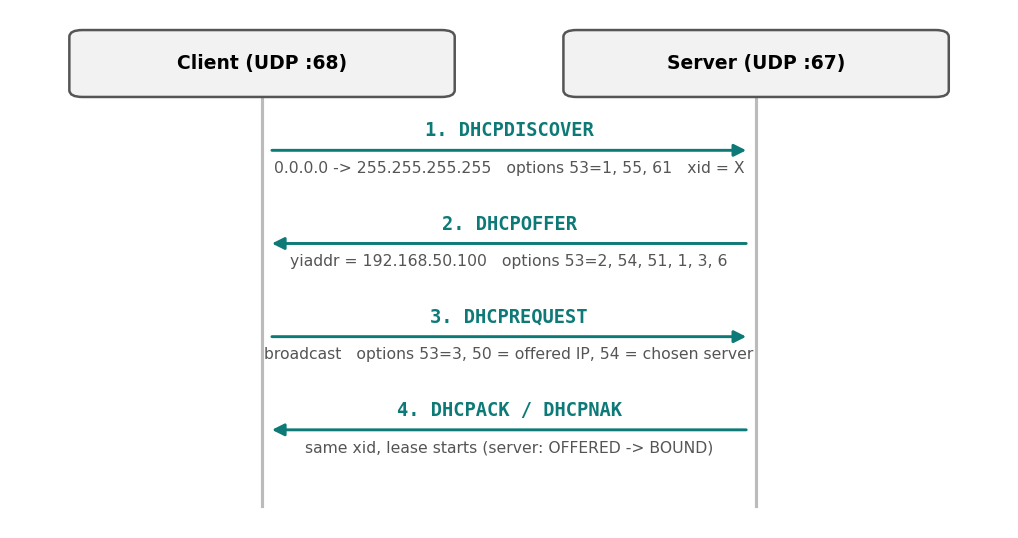
\includegraphics[width=0.82\textwidth]{figures/dhcp_dora.png}
\caption{The DHCP exchange (``DORA'') as implemented, with the options each message
carries.}
\label{fig:dora}
\end{figure}

\begin{table}[H]
\centering
\small
\begin{tabular}{rllp{7.2cm}}
\toprule
\textbf{Offset} & \textbf{Field} & \textbf{Size} & \textbf{Use in this project} \\
\midrule
0   & \texttt{op}, \texttt{htype}, \texttt{hlen}, \texttt{hops} & 1 each &
      1 = request / 2 = reply; 1 = Ethernet; 6; 0 \\
4   & \texttt{xid}    & 4   & Random transaction ID, same for the whole exchange \\
8   & \texttt{secs}, \texttt{flags} & 2, 2 & 0; 0x8000 = broadcast reply \\
12  & \texttt{ciaddr} & 4   & Client IP when renewing (0 here) \\
16  & \texttt{yiaddr} & 4   & ``Your'' IP: the offered / assigned address \\
20  & \texttt{siaddr}, \texttt{giaddr} & 4, 4 & Boot server, relay agent (0) \\
28  & \texttt{chaddr} & 16  & Client MAC in the first 6 bytes \\
44  & \texttt{sname}, \texttt{file} & 64, 128 & Unused (zero) \\
236 & magic cookie    & 4   & 0x63825363: DHCP options follow \\
240 & options         & var & \texttt{[code][length][data]}~\ldots, END (255), PAD (0) to
      300 bytes \\
\bottomrule
\end{tabular}
\caption{DHCP message format (the BOOTP header followed by options).}
\label{tab:dhcppkt}
\end{table}

\begin{table}[H]
\centering
\small
\begin{tabular}{rlp{8.6cm}}
\toprule
\textbf{Code} & \textbf{Option} & \textbf{Sent by} \\
\midrule
53  & Message type & everyone: 1 DISCOVER, 2 OFFER, 3 REQUEST, 4 DECLINE, 5 ACK, 6 NAK,
                     7 RELEASE \\
50  & Requested IP & client in REQUEST (the offered address) \\
54  & Server identifier & server in every reply; client in REQUEST (the chosen server) \\
55  & Parameter request list & client: 1, 3, 6, 51, 54 \\
61  & Client identifier & client: type 1 + MAC \\
51  & Lease time & server in OFFER/ACK \\
1, 3, 6 & Subnet mask, router, DNS & server in OFFER/ACK \\
255 & End & everyone \\
\bottomrule
\end{tabular}
\caption{DHCP options used by the client and the server.}
\label{tab:options}
\end{table}

\subsection{Design of the ARP Simulation}
\paragraph{A hub process as the Ethernet.} Sending and receiving raw Ethernet frames
requires administrator rights and different APIs on every operating system. We therefore
simulate the LAN (Figure~\ref{fig:arparch}). \texttt{lan\_hub} is a TCP server on
\texttt{127.0.0.1:9200} that plays the switch, and every host is an independent process
connected to it. Each TCP connection is a cable to one switch port. This is the same
``central medium + independent station processes'' design used in Assignments 3 and 4.
Only the transport is simulated: the packets the hosts exchange are byte-for-byte the
28-byte ARP packets of Table~\ref{tab:arppkt}, in network byte order.

\paragraph{The hub behaves like a switch.} A host first registers with a text line
\texttt{REG <ip> <mac>}, which tells the hub which MAC is behind which port, and the hub
answers \texttt{OK}. After that every message is one ARP packet. A \emph{request} is
flooded to every other port, which is a broadcast. A \emph{reply} is forwarded only to the
port whose MAC equals the packet's \texttt{tha}, which is a unicast. The hub never answers
ARP itself and never looks at a host's cache, so all protocol logic lives in the hosts.
It serves all hosts from one thread with \texttt{select()}.

\paragraph{Two threads per host.} A host must answer requests from others at any moment,
including while its user is typing or while it is waiting for its own reply. The
\emph{receiver thread} reads packets and runs the RFC~826 receive logic. The \emph{main
thread} reads commands and performs lookups. The two threads share only the ARP cache,
which is protected by a mutex, and the socket, whose sends are also serialised by a mutex.

\paragraph{Receive logic.} For every incoming packet, a host applies these checks in
order:
\begin{enumerate}[leftmargin=1.8em,itemsep=0pt]
  \item The sender claims \emph{my} IP with a different MAC: print an IP-conflict warning.
  \item Gratuitous (\texttt{spa = tpa}): refresh the sender's entry if it is already cached.
  \item A request for my IP: cache the sender, then unicast a reply.
  \item A request for someone else: refresh the sender only if it is already cached
  (the RFC~826 ``merge'' rule).
  \item A reply: cache the sender.
\end{enumerate}

\begin{figure}[H]
\centering
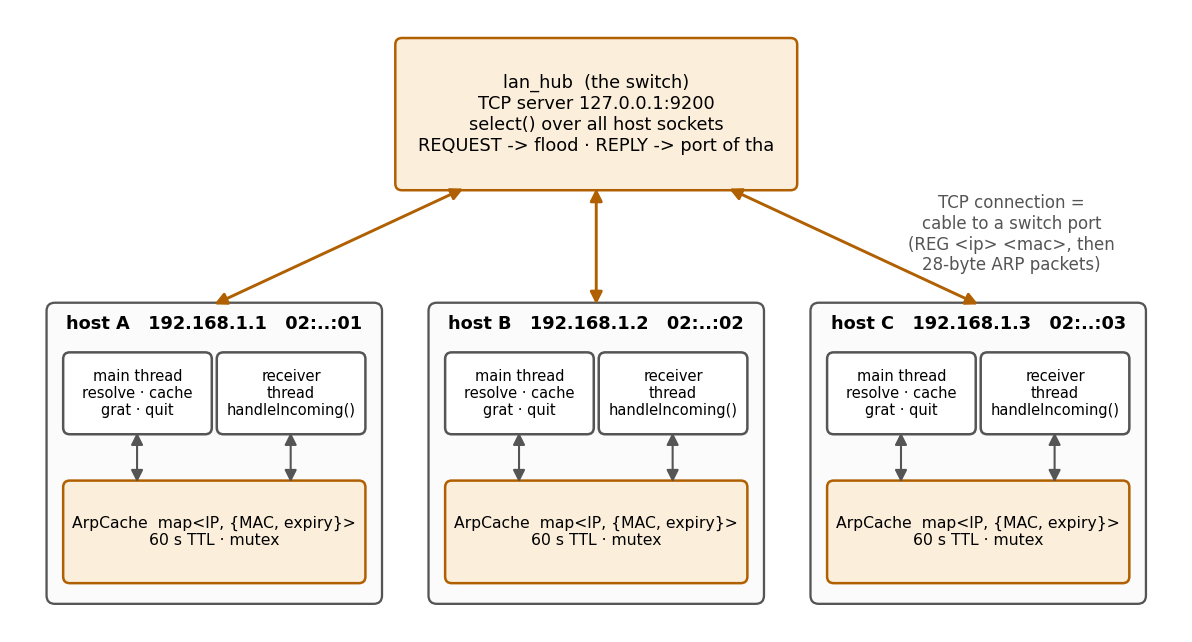
\includegraphics[width=0.92\textwidth]{figures/arp_architecture.png}
\caption{ARP simulation: one hub process and any number of host processes.}
\label{fig:arparch}
\end{figure}

\begin{figure}[H]
\centering
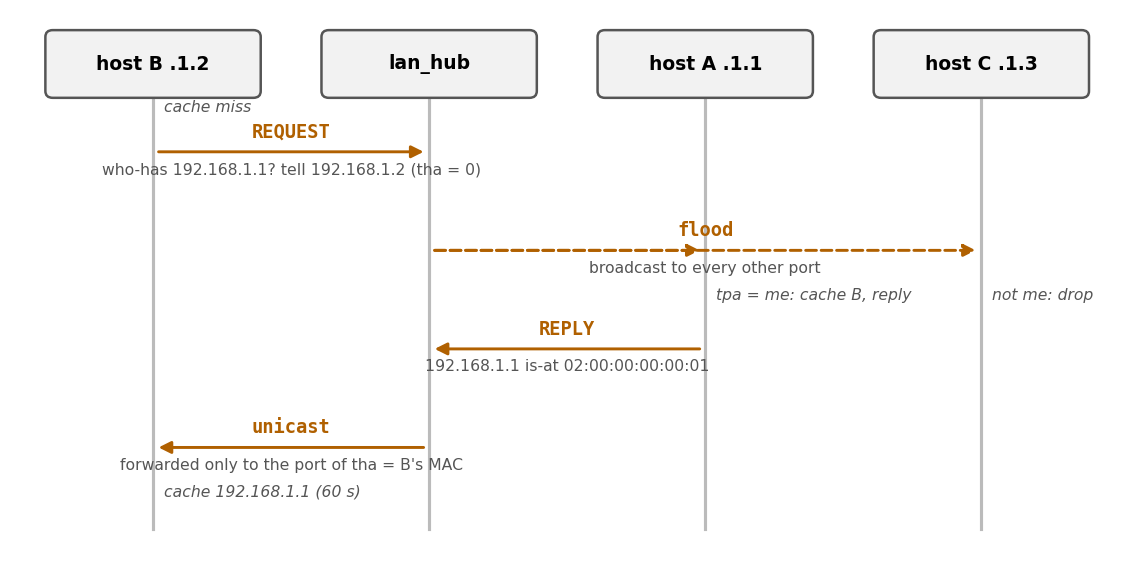
\includegraphics[width=0.85\textwidth]{figures/arp_sequence.png}
\caption{Resolving an address on a cache miss: the request is flooded, only the owner
replies, and the reply is forwarded to the requester's port alone.}
\label{fig:arpseq}
\end{figure}

\subsection{Design of the DHCP Client and Server}
\paragraph{Real DHCP packets over UDP.} Unlike ARP, DHCP is carried in UDP. The client and
the server therefore use ordinary UDP sockets on the real ports 67 and 68 and exchange
genuine DHCP messages. Our client works against any standard DHCP server (such as a home
Wi-Fi router), and our server works with standard clients (tested with BusyBox
\texttt{udhcpc}). Both programs share one header, \texttt{dhcp\_packet.h}, with the packet
layout, the constants, and the option writer and parser.

\paragraph{Client.} The client ties its socket to one interface (\texttt{SO\_BINDTODEVICE}
on Linux, \texttt{IP\_BOUND\_IF} on macOS) so the broadcast leaves through the right
network card, and binds port~68. Each of the two steps (DISCOVER $\to$ OFFER and REQUEST
$\to$ ACK) is one call to \texttt{exchange()}. It sends the message, waits up to 4\,s for a
matching reply, and retransmits with the same \texttt{xid} up to three times. A reply is
accepted only if it is a BOOTREPLY with our \texttt{xid}, our MAC in \texttt{chaddr}, the
magic cookie, well-formed options and a server identifier. For the ACK, the server must
also be the one chosen and \texttt{yiaddr} must equal the offered address. With
\texttt{--apply} (Linux), the client finishes as a real client does and configures the
interface: it sets the address with the subnet prefix and installs the default route.

\paragraph{Server.} The server is a single loop: receive a datagram, parse it, act on the
message type, print the lease table, and broadcast the reply to port~68. Leases are kept
in a table keyed by the client's MAC address, with the states of
Figure~\ref{fig:states}. An OFFER only \emph{reserves} an address for 30\,s, so that
clients that never come back, or that choose another server, cannot use up the pool. The
REQUEST turns the reservation into a lease. Table~\ref{tab:serverlogic} lists the
server's decisions.

\begin{figure}[H]
\centering
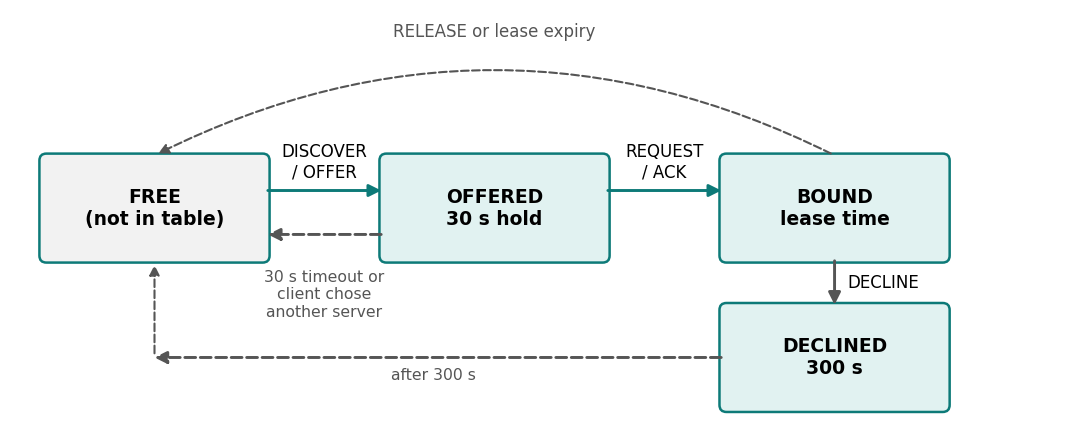
\includegraphics[width=0.85\textwidth]{figures/lease_states.png}
\caption{States of an address in the server's lease table.}
\label{fig:states}
\end{figure}

\begin{table}[H]
\centering
\small
\begin{tabular}{lp{9.2cm}l}
\toprule
\textbf{Received} & \textbf{Server's decision} & \textbf{Reply} \\
\midrule
DISCOVER & Same MAC seen before: reuse its address. Otherwise reserve the first pool
           address not in the table. Pool full: stay silent. & OFFER \\
REQUEST  & Option 54 names another server: the client chose someone else, so drop our
           reservation. & --- \\
         & Requested IP (option 50, or \texttt{ciaddr} when renewing) is this MAC's
           address: mark BOUND, start the lease. & ACK \\
         & No option 54 and no record of this MAC (a client reusing an old lease):
           RFC~2131 says stay silent. & --- \\
         & Otherwise. & NAK \\
RELEASE  & Delete the lease; the address is free again. & --- \\
DECLINE  & The client found the address in use (by ARP): block it for 300\,s. & --- \\
\bottomrule
\end{tabular}
\caption{DHCP server logic.}
\label{tab:serverlogic}
\end{table}

\paragraph{A virtual LAN for the demonstration.} A DHCP server must never be run on a
shared network: it would hand out addresses to other people's devices. The client and
server are therefore demonstrated on a virtual LAN built from three Linux kernel features
(Figure~\ref{fig:vlan}):
\begin{itemize}[leftmargin=1.6em,itemsep=0pt]
  \item A \textbf{network namespace} is a separate copy of the network stack, with its own
  interfaces, addresses, routing table, ARP cache and port numbers. Each namespace acts as
  a separate computer, while files and processes stay shared (this is the isolation that
  containers such as Docker are built on).
  \item A \textbf{veth pair} is a virtual cable: a frame sent into one end comes out of the
  other.
  \item A \textbf{bridge} is a virtual switch: it learns which MAC is behind which port,
  floods broadcasts and forwards unicast frames.
\end{itemize}
\texttt{demo.sh setup} creates a \texttt{router} namespace containing a bridge
\texttt{br0} with address 192.168.50.1/24, and three namespaces \texttt{pc1}--\texttt{pc3},
each with an \texttt{eth0} plugged into the bridge and \emph{no} IP address.
The server runs in \texttt{router}, and each client runs inside its PC with
\texttt{ip netns exec}. Because the configuration commands run by \texttt{--apply} inherit
the namespace, they configure that PC's \texttt{eth0}, not the host machine.

\begin{figure}[H]
\centering
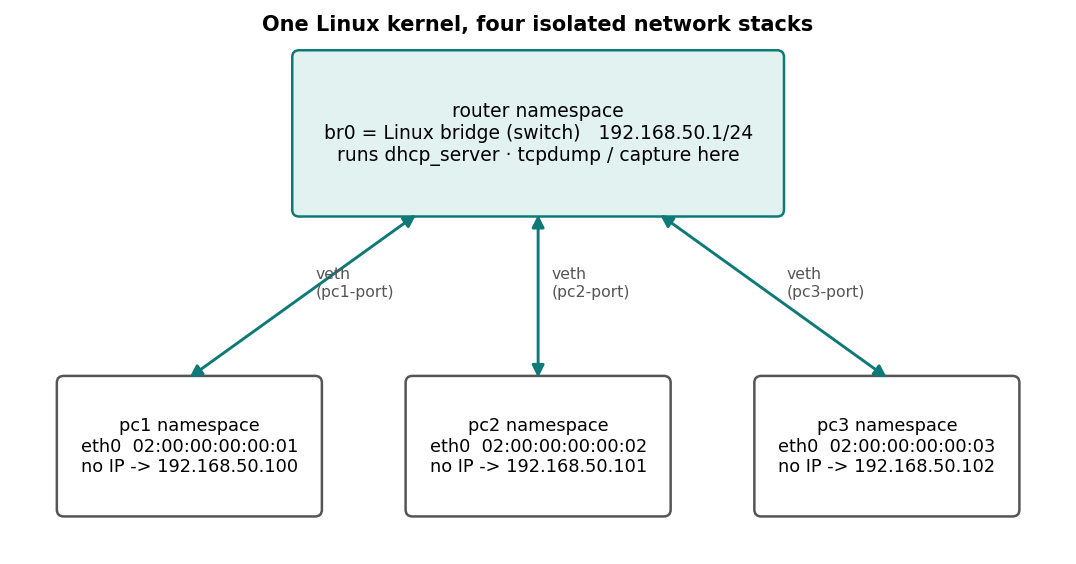
\includegraphics[width=0.78\textwidth]{figures/virtual_lan.png}
\caption{The virtual LAN created by \texttt{demo.sh setup}.}
\label{fig:vlan}
\end{figure}

\subsection{Input and Output Format}
\paragraph{ARP.} \texttt{./lan\_hub} takes no arguments and logs every packet it forwards.
\texttt{./host <myIP> <myMAC> [peerIP]} registers with the hub (resolving
\texttt{peerIP} at start-up if given) and then reads commands from standard input:
\texttt{resolve <ip>}, \texttt{cache}, \texttt{grat} and \texttt{quit}. It prints every
event: requests received, replies sent, cache updates and conflicts. For example:
\begin{lstlisting}[style=log]
ARP REQUEST who-has 192.168.1.1  tell 192.168.1.2 (02:00:00:00:00:02)  [BROADCAST]
ARP REPLY 192.168.1.1 is-at 02:00:00:00:00:01  -> 02:00:00:00:00:02  [UNICAST]
\end{lstlisting}

\paragraph{DHCP.}
\texttt{sudo ./dhcp\_server <interface> <server-ip> <pool-first> <pool-last> [lease-s]}
prints its configuration and then, for every message, the decision and the whole lease
table. \texttt{sudo ./dhcp\_client [interface] [MAC] [--apply]} lists interfaces and asks
for one when none is given, prints the OFFER and the ACK, and exits with status 0 only if
a lease was obtained. The demonstration is driven by \texttt{demo.sh}
(Table~\ref{tab:demo}).

\begin{table}[H]
\centering
\small
\begin{tabular}{lp{10.2cm}}
\toprule
\textbf{Command} & \textbf{Effect} \\
\midrule
\texttt{setup} / \texttt{cleanup} & Build / delete the virtual LAN (and compile both programs) \\
\texttt{server [lease] [n]} & Run \texttt{dhcp\_server} in the router with \texttt{n}
  addresses (default 3) \\
\texttt{client <pc>} & Run \texttt{dhcp\_client eth0 --apply} inside \texttt{<pc>} \\
\texttt{udhcpc <pc>} & Obtain a lease with BusyBox \texttt{udhcpc} instead \\
\texttt{ping <pc> [ip]} & Ping from \texttt{<pc>}, then print its ARP cache \\
\texttt{shell <machine>} & Open a shell inside a namespace (\texttt{ip a},
  \texttt{ip route}, \texttt{ip neigh}) \\
\texttt{show} / \texttt{watch} & Every machine's IP, MAC, gateway, ARP cache and the
  switch's MAC table (once / every second) \\
\texttt{capture} / \texttt{capture-file} & \texttt{tcpdump} on the switch (live / to a
  pcap file for Wireshark) \\
\texttt{reset <pc>} & Remove a PC's address so it can ask again \\
\bottomrule
\end{tabular}
\caption{Commands of \texttt{dhcp/demo.sh} (all run with \texttt{sudo}).}
\label{tab:demo}
\end{table}

\section{Implementation}
Both parts are written in C++17 with BSD sockets. The demonstration and experiment
tooling is in Bash and Python.

\subsection{Component Breakdown}
\begin{itemize}[leftmargin=1.6em]
  \item \texttt{arp/arp\_packet.h}: the \texttt{ArpPacket} struct (packed, 28 bytes,
  checked by \texttt{static\_assert}), the request, reply and gratuitous builders, and the
  parse/print helpers for IP and MAC addresses.
  \item \texttt{arp/portable\_net.h}: small socket shims for Windows and POSIX, and
  \texttt{recvAll()}.
  \item \texttt{arp/lan\_hub.cpp}: the switch (registration, flooding, forwarding by MAC).
  \item \texttt{arp/host.cpp}: a host (command loop, receiver thread, ARP cache).
  \item \texttt{dhcp/dhcp\_packet.h}: the DHCP message struct, constants, and the option
  writer (\texttt{addOption}, \texttt{finishOptions}) and parser (\texttt{parseOptions}),
  shared by client and server.
  \item \texttt{dhcp/Dhcp.cpp}: the client (Linux and macOS).
  \item \texttt{dhcp/DhcpServer.cpp}: the server (pool, lease table, replies).
  \item \texttt{dhcp/demo.sh}, \texttt{dhcp/udhcpc\_hook.sh}: the virtual LAN and the
  demonstration commands.
  \item \texttt{experiments/run\_experiments.py}: every test and measurement in
  \S\ref{sec:tests}--\S\ref{sec:results}, writing \texttt{results/*.csv}.
  \item \texttt{report/make\_figures.py}: every figure in this report.
\end{itemize}

\begin{figure}[H]
\centering
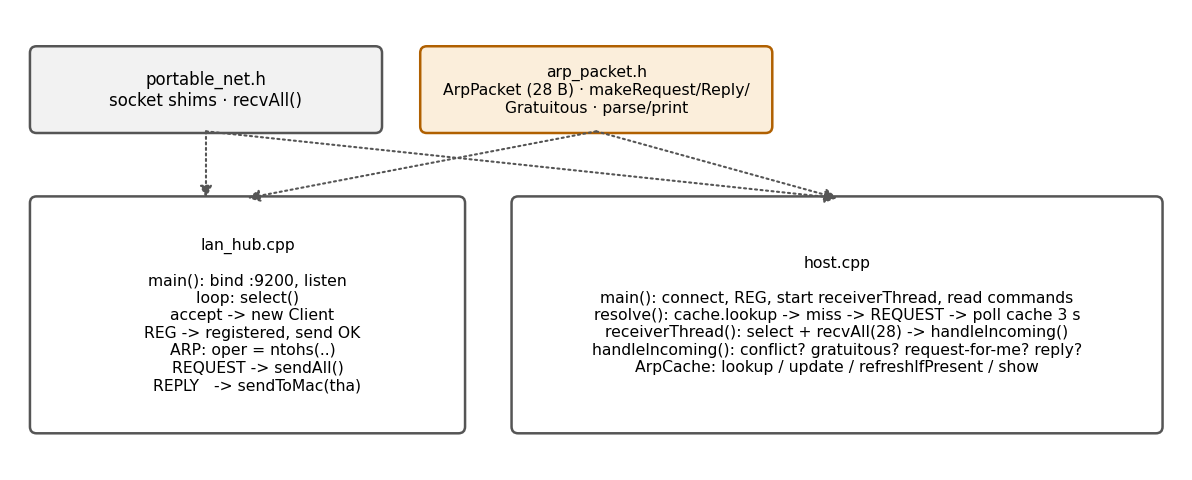
\includegraphics[width=0.95\textwidth]{figures/arp_structure.png}
\caption{Procedural structure of the ARP simulation.}
\label{fig:arpstruct}
\end{figure}

\begin{figure}[H]
\centering
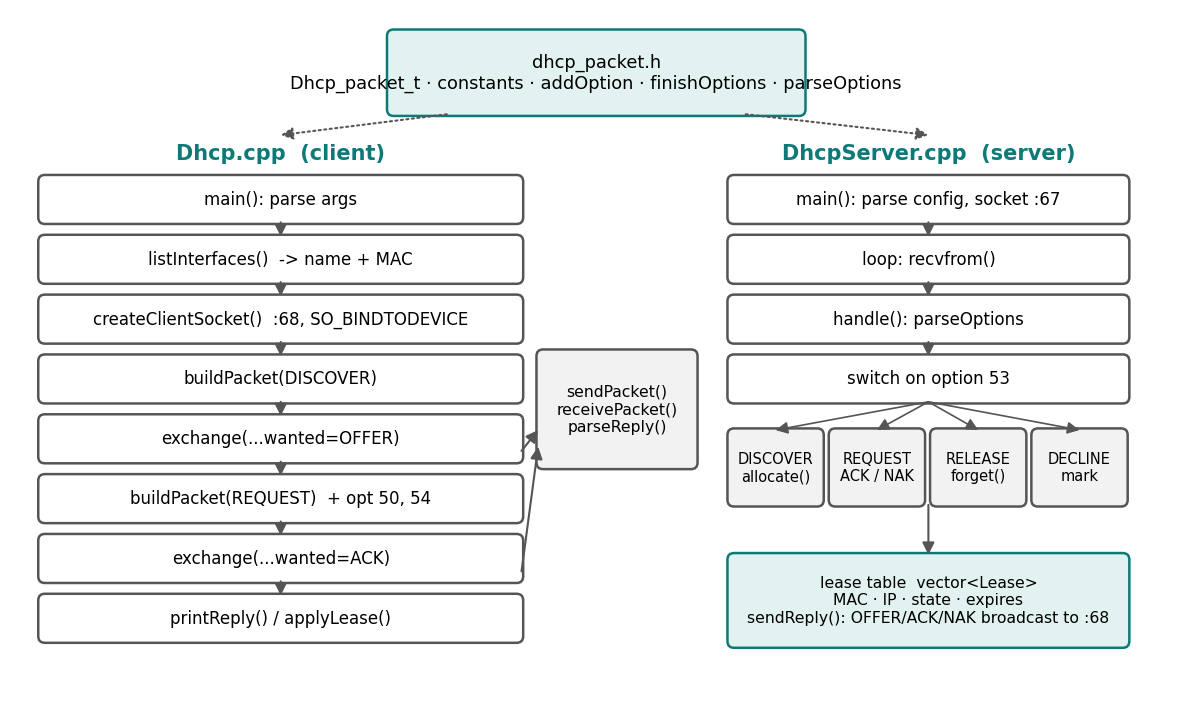
\includegraphics[width=\textwidth]{figures/dhcp_structure.png}
\caption{Procedural structure of the DHCP client and server.}
\label{fig:dhcpstruct}
\end{figure}

\subsection{ARP: Building a Request}
\begin{lstlisting}
inline void makeRequest(ArpPacket& p, const unsigned char sha[6],
                        const unsigned char spa[4], const unsigned char tpa[4]) {
    memset(&p, 0, sizeof(p));
    p.htype = htons(1);          // Ethernet       (network byte order on the wire)
    p.ptype = htons(0x0800);     // IPv4
    p.hlen = 6;  p.plen = 4;
    p.oper = htons(ARP_REQUEST);
    setMac(p.sha, sha);  setIp(p.spa, spa);
    zeroMac(p.tha);              // unknown: that is the question
    setIp(p.tpa, tpa);
}
// Gratuitous ARP = a request for one's own address: makeRequest(p, myMac, myIp, myIp)
\end{lstlisting}

\subsection{ARP: Framing on the TCP ``Cable''}
TCP delivers a byte stream, not messages. A single \texttt{recv()} may return half a
packet, or two packets joined together. Both the hub and the hosts therefore read exactly
one 28-byte packet at a time:
\begin{lstlisting}
inline int recvAll(SOCKET s, char* buf, int len) {
    int got = 0;
    while (got < len) {
        int n = recv(s, buf + got, len - got, 0);
        if (n <= 0) return n;          // peer left
        got += n;
    }
    return got;
}
\end{lstlisting}

\subsection{ARP: The Hub's Forwarding Decision}
\begin{lstlisting}
ArpPacket pkt;
memcpy(&pkt, buf, sizeof(pkt));
unsigned short oper = ntohs(pkt.oper);
if (oper == ARP_REQUEST)
    sendAll(clients, buf, sizeof(ArpPacket), s);          // flood to every other port
else if (oper == ARP_REPLY)
    sendToMac(clients, pkt.tha, buf, sizeof(ArpPacket));  // only the port owning tha
\end{lstlisting}

\subsection{ARP: Receive Logic of a Host}
\begin{lstlisting}
void handleIncoming(const ArpPacket& pkt) {
    unsigned short oper = ntohs(pkt.oper);
    bool gratuitous = (oper == ARP_REQUEST && memcmp(pkt.spa, pkt.tpa, 4) == 0);

    if (memcmp(pkt.spa, gMyIp, 4) == 0 && memcmp(pkt.sha, gMyMac, 6) != 0) {
        cout << "  [WARNING] IP conflict: " << macToStr(pkt.sha) << " also claims "
             << ipToStr(gMyIp) << "\n";
        return;
    }
    if (gratuitous) {                                   // announce: refresh if known
        cache.refreshIfPresent(pkt.spa, pkt.sha);
        return;
    }
    if (oper == ARP_REQUEST) {
        if (memcmp(pkt.tpa, gMyIp, 4) != 0) {           // not for me: merge only
            cache.refreshIfPresent(pkt.spa, pkt.sha);
            return;
        }
        cache.update(pkt.spa, pkt.sha);                 // the asker will talk to us
        ArpPacket rep;
        makeReply(rep, gMyMac, gMyIp, pkt.sha, pkt.spa);
        sendPacket(rep);
    } else if (oper == ARP_REPLY) {
        cache.update(pkt.spa, pkt.sha);
    }
}
\end{lstlisting}

\subsection{ARP: Lookup with Timeout}
\begin{lstlisting}
bool resolve(const unsigned char targetIp[4]) {
    unsigned char mac[6];
    if (cache.lookup(targetIp, mac)) return true;          // cache hit: nothing sent
    ArpPacket req;
    makeRequest(req, gMyMac, gMyIp, targetIp);
    sendPacket(req);                                       // broadcast
    auto deadline = steady_clock::now() + seconds(3);
    while (steady_clock::now() < deadline) {               // receiver thread fills cache
        if (cache.lookup(targetIp, mac)) return true;
        sleep_ms(50);
    }
    return false;                                          // "ARP timeout - no reply"
}
\end{lstlisting}
\texttt{ArpCache::lookup()} deletes an entry whose expiry time (insert time + 60\,s) has
passed, so an expired mapping is never returned.

\subsection{DHCP: Building DISCOVER and REQUEST}
\begin{lstlisting}
std::size_t buildPacket(Dhcp_packet_t& p, uint8_t messageType, const ClientContext& client) {
    p = {};
    p.op = BOOTREQUEST;  p.htype = 1;  p.hlen = 6;
    p.xid = htonl(client.transactionId);
    p.flags = htons(0x8000);                    // ask the server to broadcast its reply
    std::memcpy(p.chaddr, client.mac, 6);
    p.magic_cookie = htonl(DHCP_MAGIC_COOKIE);

    std::size_t i = 0;
    addOption(p, i, OPT_MSG_TYPE, &messageType, 1);
    if (messageType == DHCPREQUEST) {           // which offer we accept, and from whom
        addOption(p, i, OPT_REQUESTED_IP, &client.offeredIp, 4);
        addOption(p, i, OPT_SERVER_ID, &client.serverIp, 4);
    }
    const uint8_t wanted[] = {OPT_SUBNET_MASK, OPT_ROUTER, OPT_DNS_SERVER,
                              OPT_LEASE_TIME, OPT_SERVER_ID};
    addOption(p, i, OPT_PARAM_LIST, wanted, sizeof(wanted));
    uint8_t clientId[7] = {1};                  // type 1 (Ethernet) + MAC
    std::memcpy(clientId + 1, client.mac, 6);
    addOption(p, i, OPT_CLIENT_ID, clientId, sizeof(clientId));
    return finishOptions(p, i);                 // END + PAD up to 300 bytes
}
\end{lstlisting}
The struct needs no \texttt{\#pragma pack}, because every field already lies on its
natural alignment. Two \texttt{static\_assert}s prove that the magic cookie is at
offset~236 and the options start at offset~240.

\subsection{DHCP: Parsing Options Safely}
The parser is shared by client and server. It never reads past the bytes actually
received, and it rejects a packet without an END option:
\begin{lstlisting}
inline bool parseOptions(const Dhcp_packet_t& p, std::size_t length, DhcpOptions& out) {
    if (length < HEADER_LEN || length > sizeof(p) ||
        ntohl(p.magic_cookie) != DHCP_MAGIC_COOKIE) return false;
    out = DhcpOptions{};
    const std::size_t end = length - HEADER_LEN;
    for (std::size_t i = 0; i < end;) {
        uint8_t code = p.options[i++];
        if (code == OPT_PAD) continue;
        if (code == OPT_END) return true;
        if (i >= end) return false;              // no length byte
        uint8_t len = p.options[i++];
        if (len > end - i) return false;         // data runs past the packet
        out.data[code] = p.options + i;          // remember where each option is
        out.len[code] = len;
        i += len;
    }
    return false;                                // no END option
}
\end{lstlisting}

\subsection{DHCP: Send, Wait and Retransmit (Client)}
\begin{lstlisting}
bool exchange(int sock, const Dhcp_packet_t& packet, std::size_t length,
              const ClientContext& client, uint8_t wantedType, ParsedReply& reply) {
    for (int attempt = 1; attempt <= 3; ++attempt) {
        if (!sendPacket(sock, packet, length)) return false;  // to 255.255.255.255:67
        auto deadline = Clock::now() + std::chrono::seconds(4);
        while (Clock::now() < deadline) {
            Dhcp_packet_t response{};
            int n = receivePacket(sock, response);            // 1 s socket timeout
            if (n < 0) return false;
            if (n == 0 || !parseReply(response, n, client, reply)) continue;
            if (wantedType == DHCPOFFER && reply.messageType == DHCPOFFER) return true;
            if (wantedType == DHCPACK && reply.serverIp == client.serverIp) {
                if (reply.messageType == DHCPNAK) return true;
                if (reply.messageType == DHCPACK && reply.offeredIp == client.offeredIp)
                    return true;
            }
        }
    }
    return false;
}
\end{lstlisting}

\subsection{DHCP: Address Allocation and REQUEST Handling (Server)}
\begin{lstlisting}
Lease* allocate(const uint8_t* mac) {
    removeExpired();
    if (Lease* existing = findByMac(mac)) return existing;    // same MAC, same IP
    for (uint32_t ip = cfg.poolFirst; ip <= cfg.poolLast; ++ip) {
        if (ipInUse(ip)) continue;
        Lease l{};
        std::memcpy(l.mac, mac, 6);
        l.ip = ip;
        l.state = State::Offered;
        l.expires = std::time(nullptr) + OFFER_HOLD_SECONDS;  // 30 s reservation
        leases.push_back(l);
        return &leases.back();
    }
    return nullptr;                                           // pool exhausted
}

case DHCPREQUEST: {
    uint32_t serverId = ntohl(o.ip(OPT_SERVER_ID));
    if (o.has(OPT_SERVER_ID) && serverId != cfg.serverIp) {   // chose another server
        Lease* l = findByMac(mac);
        if (l && l->state == State::Offered) forget(mac);
        break;
    }
    uint32_t wanted = ntohl(o.has(OPT_REQUESTED_IP) ? o.ip(OPT_REQUESTED_IP) : p.ciaddr);
    Lease* l = findByMac(mac);
    if (l && l->ip == wanted) {
        l->state = State::Bound;
        l->expires = std::time(nullptr) + cfg.leaseSeconds;
        sendReply(sock, p, DHCPACK, l->ip);
    } else if (!l && !o.has(OPT_SERVER_ID)) {
        return;                                               // RFC 2131: stay silent
    } else {
        sendReply(sock, p, DHCPNAK, 0);
    }
    break;
}
\end{lstlisting}
\texttt{sendReply()} copies \texttt{xid}, \texttt{flags} and \texttt{chaddr} from the
request, writes the address into \texttt{yiaddr}, adds options 53, 54, 51, 1, 3 and~6
(only 53 and 54 for a NAK), and broadcasts the result to \texttt{255.255.255.255:68}.

\subsection{DHCP: Applying the Lease and Building the Virtual LAN}
With \texttt{--apply} the client converts the subnet mask into a prefix length and runs
\texttt{ip addr flush dev eth0 \&\& ip addr add <ip>/<prefix> dev eth0 \&\& ip route
replace default via <router>}. The interface name is first checked to contain only
letters, digits, \texttt{-}, \texttt{\_} and~\texttt{.}, because it is inserted into a
shell command. The core of \texttt{demo.sh setup}:
\begin{lstlisting}[language=bash]
ip netns add router
ip -n router link add br0 type bridge                     # the switch
ip -n router addr add 192.168.50.1/24 dev br0
for pc in pc1 pc2 pc3; do
    ip netns add "$pc"
    ip link add "tmp-$pc" type veth peer name "$pc-port"   # a cable
    ip link set "tmp-$pc" netns "$pc"                      # one end into the PC ...
    ip -n "$pc" link set "tmp-$pc" name eth0
    ip link set "$pc-port" netns router                    # ... the other into the switch
    ip -n router link set "$pc-port" master br0 up
    ip netns exec "$pc" sysctl -qw net.ipv4.conf.all.rp_filter=0 \
                                   net.ipv4.conf.eth0.rp_filter=0
done
\end{lstlisting}
The last line is needed because the client uses an ordinary UDP socket. When the OFFER
arrives the PC has no address and no routes, and Linux's reverse-path filter would drop a
packet it has no route back for. Real clients avoid this with raw packet sockets. Here
the check is disabled inside the PC namespaces only.

\subsection{Performance Metrics}
\begin{itemize}[leftmargin=1.6em]
  \item \textbf{Correctness}: each functional test either produces the expected address,
  reply or log line, or it does not (PASS/FAIL).
  \item \textbf{Lease success rate}: fraction of client runs that end with an ACK, under a
  given packet-loss rate.
  \item \textbf{Time to lease}: wall-clock time from starting the client to the ACK.
  \item \textbf{Retransmissions}: DISCOVER and REQUEST messages sent per run.
  \item \textbf{ARP requests and frames on the LAN}: requests sent, and frames the hub
  delivers, to resolve every host from every other host. Measured with an empty cache and
  again with a warm cache.
\end{itemize}

\section{Test Cases}
\label{sec:tests}
All tests are automated in \texttt{experiments/run\_experiments.py}. It runs with
\texttt{sudo}, or without it inside an unprivileged user and network namespace
(\texttt{unshare -rnm}), which behaves the same for everything tested here.

\subsection{ARP}
\begin{itemize}[leftmargin=1.6em]
  \item \textbf{A1: Resolution on a cache miss.} Host B (192.168.1.2) starts with peer
  192.168.1.1. \emph{Checking:} B broadcasts a request, the hub floods it, A caches B and
  replies, the hub forwards the reply to B's port only, and B prints
  \emph{Resolved (after reply)}.
  \item \textbf{A2: Cache hit.} B resolves 192.168.1.1 again. \emph{Checking:}
  \emph{Resolved (cache hit)}, and the hub logs no packet.
  \item \textbf{A3: Unknown address.} B resolves 192.168.1.9 (no such host).
  \emph{Checking:} one broadcast, then \emph{ARP timeout -- no reply} after 3\,s; the
  cache is unchanged.
  \item \textbf{A4: Gratuitous ARP refreshes caches.} A sends \texttt{grat}.
  \emph{Checking:} the hub labels it \emph{(gratuitous)}; B, which has A cached,
  refreshes the entry to a full 60\,s.
  \item \textbf{A5: IP conflict and ARP spoofing.} A third host claims 192.168.1.1 with MAC
  \texttt{02:00:00:00:00:99} and sends \texttt{grat}. \emph{Checking:} A prints an
  IP-conflict warning; B's cache now maps 192.168.1.1 to the new MAC.
  \item \textbf{A6: Cache behaviour at scale.} $N=2\ldots8$ hosts; every host resolves
  every other host, twice. \emph{Checking:} the number of requests in each round matches
  the analysis in \S\ref{sec:arpanalysis}.
  \item \textbf{A7: Framing.} A test client sends two ARP requests in a single
  \texttt{send()}. \emph{Checking:} the hub forwards both and both owners reply. (The earlier hub read up to 512 bytes per
  \texttt{recv()} and processed only the first packet in the buffer.)
\end{itemize}

\subsection{DHCP: Functional Tests on the Virtual LAN}
Table~\ref{tab:functional} lists the 13 functional tests and their outcomes. Tests F5--F11
use hand-made DHCP messages sent from a PC namespace, so that server behaviour our own
client never triggers (a NAK, a REQUEST for another server, RELEASE, DECLINE, a malformed
packet) can be checked as well.

\subsection{DHCP: Robustness Under Packet Loss}
\textbf{L1.} The Linux traffic shaper \texttt{netem} drops a fixed percentage
$p\in\{0,10,20,30,40,50\}\%$ of the packets on pc1's cable, in both directions. The client
is run 30 times at each level. \emph{Checking:} leases are still obtained thanks to
retransmission, and the success rate and time to lease agree with the model of
\S\ref{sec:lossanalysis}.

\subsection{Whole-System Check: Capture on the Switch}
\textbf{C1.} A raw capture on \texttt{br0} while pc1 and pc2 obtain leases and then ping
the router and each other. \emph{Checking:} the frames on the wire are exactly the
DORA exchange, then ARP request/reply, then ICMP. They are decoded correctly by
\texttt{tcpdump} (an independent DHCP and ARP decoder), and the source of DISCOVER is
\texttt{0.0.0.0}.

\section{Results}
\label{sec:results}

\subsection{ARP Scenario (A1--A5)}
Host B's output (from \texttt{results/arp\_hostB.log}):
\begin{lstlisting}[style=log]
=== Resolve peer 192.168.1.1 ===
  Cache miss for 192.168.1.1
  Sending ARP REQUEST (broadcast): who-has 192.168.1.1?
  [event] ARP REPLY 192.168.1.1 is-at 02:00:00:00:00:01
  [cache] 192.168.1.1 -> 02:00:00:00:00:01  (ttl 60s)
  Resolved (after reply): 192.168.1.1 -> 02:00:00:00:00:01
  Resolved (cache hit): 192.168.1.1 -> 02:00:00:00:00:01
  Cache miss for 192.168.1.9
  Sending ARP REQUEST (broadcast): who-has 192.168.1.9?
  ARP timeout - no reply
  --- ARP Cache ---
  192.168.1.1  02:00:00:00:00:01  remaining=55s
  [event] Gratuitous ARP: 192.168.1.1 is-at 02:00:00:00:00:01
  [cache] 192.168.1.1 -> 02:00:00:00:00:01  (ttl 60s)
  [event] Gratuitous ARP: 192.168.1.1 is-at 02:00:00:00:00:99
  [cache] 192.168.1.1 -> 02:00:00:00:00:99  (ttl 60s)
  --- ARP Cache ---
  192.168.1.1  02:00:00:00:00:99  remaining=60s
\end{lstlisting}
Host A's output, and the hub's log of the same run:
\begin{lstlisting}[style=log]
  [event] ARP REQUEST who-has ME from 192.168.1.2 (02:00:00:00:00:02)
  [cache] 192.168.1.2 -> 02:00:00:00:00:02  (ttl 60s)
  [event] ARP REPLY sent: 192.168.1.1 is-at 02:00:00:00:00:01
  Gratuitous ARP announced for 192.168.1.1
  [WARNING] IP conflict: 02:00:00:00:00:99 also claims 192.168.1.1

ARP REQUEST who-has 192.168.1.1  tell 192.168.1.2 (02:00:00:00:00:02)  [BROADCAST]
ARP REPLY 192.168.1.1 is-at 02:00:00:00:00:01  -> 02:00:00:00:00:02  [UNICAST]
ARP REQUEST who-has 192.168.1.9  tell 192.168.1.2 (02:00:00:00:00:02)  [BROADCAST]
ARP REQUEST who-has 192.168.1.1  tell 192.168.1.1 (02:00:00:00:00:01)  [BROADCAST] (gratuitous)
ARP REQUEST who-has 192.168.1.1  tell 192.168.1.1 (02:00:00:00:00:99)  [BROADCAST] (gratuitous)
\end{lstlisting}
All five behaviours appear as expected. The cache hit (A2) produced no line in the hub
log, and the request for 192.168.1.9 (A3) received no reply.

\subsection{ARP Traffic with and without the Cache (A6)}
\begin{table}[H]
\centering
\small
\setlength{\tabcolsep}{5pt}
\begin{tabular}{rrrrrrr}
\toprule
& & \multicolumn{2}{c}{\textbf{Round 1 (empty caches)}} &
  \multicolumn{2}{c}{\textbf{Round 2 (warm caches)}} & \\
\cmidrule(lr){3-4}\cmidrule(lr){5-6}
\textbf{N} & \textbf{Lookups/round} & \textbf{Requests} & \textbf{Replies} &
\textbf{Requests} & \textbf{Replies} & \textbf{Frames, round 1} \\
\midrule
2 & 2 & 1 & 1 & 0 & 0 & 2 \\
3 & 6 & 3 & 3 & 0 & 0 & 9 \\
4 & 12 & 6 & 6 & 0 & 0 & 24 \\
5 & 20 & 10 & 10 & 0 & 0 & 50 \\
6 & 30 & 15 & 15 & 0 & 0 & 90 \\
7 & 42 & 21 & 21 & 0 & 0 & 147 \\
8 & 56 & 28 & 28 & 0 & 0 & 224 \\
\bottomrule
\end{tabular}
\caption{Every host resolves every other host, twice. Requests and replies are counted
from the hub's log. ``Frames, round 1'' is the number of frames the hub delivers:
$N-1$ flooded copies of each request plus one copy of each reply.}
\label{tab:arptraffic}
\end{table}

\begin{figure}[H]
\centering
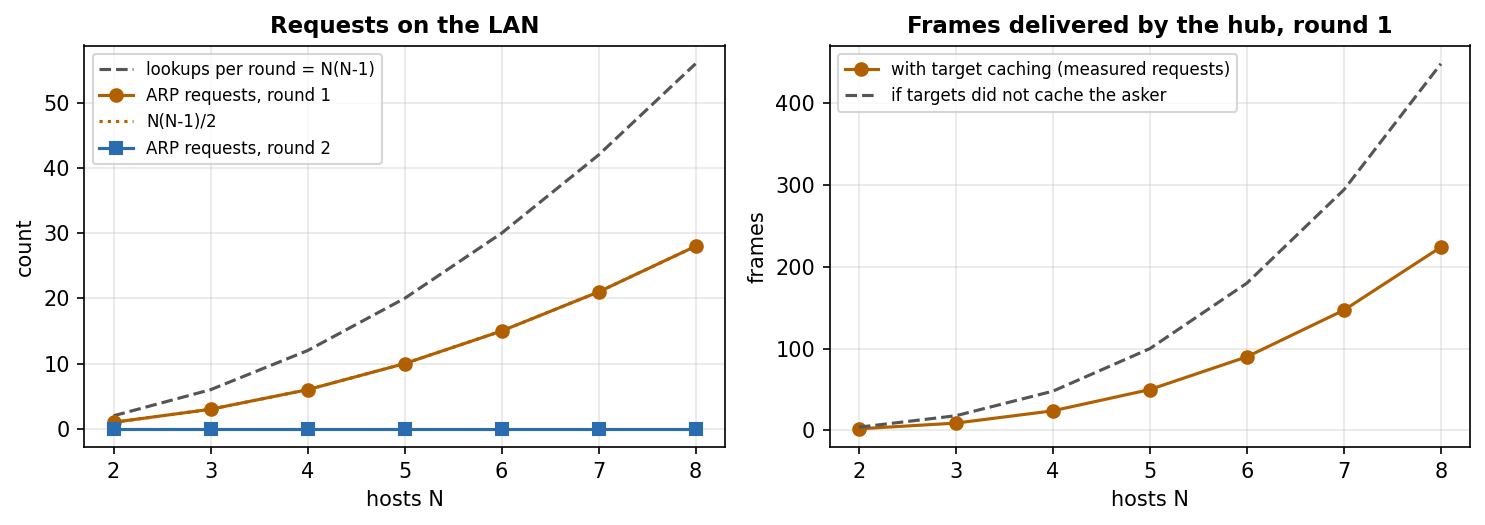
\includegraphics[width=0.95\textwidth]{figures/arp_traffic.png}
\caption{Left: ARP requests per round. Right: frames the hub must deliver in round 1,
compared with the traffic if the target of a request did not cache the requester.}
\label{fig:arptraffic}
\end{figure}

\subsection{DHCP Functional Tests (F1--F13)}
\begin{table}[H]
\centering
\small
\begin{tabular}{lp{8.3cm}lll}
\toprule
\textbf{ID} & \textbf{Test} & \textbf{Expected} & \textbf{Observed} & \textbf{Result} \\
\midrule
F1 & pc1 obtains a lease & .100 & .100 & \textbf{PASS} \\
F2 & pc2 (different MAC) gets the next address & .101 & .101 & \textbf{PASS} \\
F3 & pc1 asks again: same MAC, same address & .100 & .100 & \textbf{PASS} \\
F4 & BusyBox udhcpc (independent client) on pc3 & .102 & .102 & \textbf{PASS} \\
F5 & REQUEST for an address not reserved for this MAC & NAK & NAK & \textbf{PASS} \\
F6 & REQUEST naming another server (offer withdrawn) & none & none & \textbf{PASS} \\
F7 & INIT-REBOOT REQUEST from an unknown client (RFC: stay silent) & none & none & \textbf{PASS} \\
F8 & malformed packet (option runs past the end) is ignored & none & none & \textbf{PASS} \\
F9 & pool full (3 of 3 bound): DISCOVER from a 4th MAC & none & none & \textbf{PASS} \\
F10 & after pc2 sends RELEASE, the 4th MAC gets an OFFER & OFFER & OFFER & \textbf{PASS} \\
F11 & after pc3 DECLINEs .102, .102 is blocked (pool now full) & no lease & no lease & \textbf{PASS} \\
F12 & server logged the DECLINE and the pool-exhausted case & yes & yes & \textbf{PASS} \\
F13 & client with a non-existent interface exits with an error & 1 & 1 & \textbf{PASS} \\
\bottomrule
\end{tabular}
\caption{DHCP functional tests on the virtual LAN (pool 192.168.50.100--102). ``none''
means no reply within 2\,s.}
\label{tab:functional}
\end{table}

\subsection{A Complete Lease}
Client output for pc1 (\texttt{sudo ./demo.sh client pc1}):
\begin{lstlisting}[style=log]
Using interface eth0, MAC 02:00:00:00:00:01
Sent DHCPDISCOVER (300 bytes, XID 0x35879470), attempt 1/3
Received 300 bytes from 192.168.50.1:67
---- DHCPOFFER ----
  Server ID   : 192.168.50.1
  Your IP     : 192.168.50.100
  Subnet mask : 255.255.255.0
  Router      : 192.168.50.1
  DNS server  : 8.8.8.8
  Lease       : 120 seconds
Sent DHCPREQUEST (300 bytes, XID 0x35879470), attempt 1/3
Received 300 bytes from 192.168.50.1:67
---- DHCPACK ----
  (same values as the OFFER)
Applying: ip addr flush dev eth0 && ip addr add 192.168.50.100/24 dev eth0 && ip route replace default via 192.168.50.1 dev eth0
Interface eth0 is now configured.
\end{lstlisting}
The server's log for pc1 and pc2:
\begin{lstlisting}[style=log]
DHCP server 192.168.50.1 on br0
  pool 192.168.50.100 - 192.168.50.102, mask 255.255.255.0, router 192.168.50.1, DNS 8.8.8.8, lease 120s
<- DHCPDISCOVER from 02:00:00:00:00:01 (xid 0x35879470)
  -> DHCPOFFER 192.168.50.100 to 02:00:00:00:00:01
  | 02:00:00:00:00:01 | 192.168.50.100  | OFFERED  |    30s  |
<- DHCPREQUEST from 02:00:00:00:00:01 (xid 0x35879470)
  -> DHCPACK 192.168.50.100 to 02:00:00:00:00:01
  | 02:00:00:00:00:01 | 192.168.50.100  | BOUND    |   120s  |
<- DHCPDISCOVER from 02:00:00:00:00:02 (xid 0xfd207410)
  -> DHCPOFFER 192.168.50.101 to 02:00:00:00:00:02
  | 02:00:00:00:00:01 | 192.168.50.100  | BOUND    |   119s  |
  | 02:00:00:00:00:02 | 192.168.50.101  | OFFERED  |    30s  |
<- DHCPREQUEST from 02:00:00:00:00:02 (xid 0xfd207410)
  -> DHCPACK 192.168.50.101 to 02:00:00:00:00:02
  | 02:00:00:00:00:01 | 192.168.50.100  | BOUND    |   119s  |
  | 02:00:00:00:00:02 | 192.168.50.101  | BOUND    |   120s  |
\end{lstlisting}
The state of the whole LAN afterwards (\texttt{sudo ./demo.sh show}), once pc1 had pinged
the router and pc2 had pinged pc1. The addresses come from DHCP, and the ARP caches and
the switch's MAC table were filled by the Linux kernel:
\begin{lstlisting}[style=log]
router  br0   IP 192.168.50.1/24    MAC 22:41:6d:21:e5:fe
          ARP cache: 192.168.50.100 -> 02:00:00:00:00:01 DELAY
pc1     eth0  IP 192.168.50.100/24  MAC 02:00:00:00:00:01   gateway 192.168.50.1
          ARP cache: 192.168.50.101 -> 02:00:00:00:00:02 DELAY | 192.168.50.1 -> 22:41:6d:21:e5:fe REACHABLE
pc2     eth0  IP 192.168.50.101/24  MAC 02:00:00:00:00:02   gateway 192.168.50.1
          ARP cache: 192.168.50.100 -> 02:00:00:00:00:01 REACHABLE
pc3     eth0  IP (no IP)            MAC 02:00:00:00:00:03
          ARP cache: (empty)
Switch (br0) MAC table: which MAC was seen on which port
          02:00:00:00:00:01  on  pc1-port
          02:00:00:00:00:02  on  pc2-port
          02:00:00:00:00:03  on  pc3-port
\end{lstlisting}

\subsection{Capture on the Virtual Switch (C1)}
\texttt{tcpdump -n -e -r results/dhcp\_arp\_capture.pcap 'not ip6'} (timestamps and some
fields shortened):
\begin{lstlisting}[style=log]
.992786 02:00:00:00:00:01 > ff:ff:ff:ff:ff:ff IPv4 342: 0.0.0.0.68 > 255.255.255.255.67: BOOTP/DHCP, Request
.992934 22:41:6d:21:e5:fe > ff:ff:ff:ff:ff:ff IPv4 342: 192.168.50.1.67 > 255.255.255.255.68: BOOTP/DHCP, Reply
.993063 02:00:00:00:00:01 > ff:ff:ff:ff:ff:ff IPv4 342: 0.0.0.0.68 > 255.255.255.255.67: BOOTP/DHCP, Request
.993099 22:41:6d:21:e5:fe > ff:ff:ff:ff:ff:ff IPv4 342: 192.168.50.1.67 > 255.255.255.255.68: BOOTP/DHCP, Reply
   ... the same four frames for pc2 (02:00:00:00:00:02) ...
.137130 02:00:00:00:00:01 > ff:ff:ff:ff:ff:ff ARP 42: Request who-has 192.168.50.1 tell 192.168.50.100
.137268 22:41:6d:21:e5:fe > 02:00:00:00:00:01 ARP 42: Reply 192.168.50.1 is-at 22:41:6d:21:e5:fe
.137295 02:00:00:00:00:01 > 22:41:6d:21:e5:fe IPv4 98: 192.168.50.100 > 192.168.50.1: ICMP echo request
.137311 22:41:6d:21:e5:fe > 02:00:00:00:00:01 IPv4 98: 192.168.50.1 > 192.168.50.100: ICMP echo reply
.207110 02:00:00:00:00:02 > ff:ff:ff:ff:ff:ff ARP 42: Request who-has 192.168.50.100 tell 192.168.50.101
\end{lstlisting}
The verbose decode of our server's OFFER (\texttt{tcpdump -vv}):
\begin{lstlisting}[style=log]
192.168.50.1.67 > 255.255.255.255.68: BOOTP/DHCP, Reply, length 300, xid 0x35879470, Flags [Broadcast] (0x8000)
  Your-IP 192.168.50.100
  Client-Ethernet-Address 02:00:00:00:00:01
  Vendor-rfc1048 Extensions
    Magic Cookie 0x63825363
    DHCP-Message (53), length 1: Offer
    Server-ID (54), length 4: 192.168.50.1
    Lease-Time (51), length 4: 120
    Subnet-Mask (1), length 4: 255.255.255.0
    Default-Gateway (3), length 4: 192.168.50.1
    Domain-Name-Server (6), length 4: 8.8.8.8
\end{lstlisting}

\subsection{DHCP Under Packet Loss (L1)}
\begin{table}[H]
\centering
\small
\setlength{\tabcolsep}{4pt}
\begin{tabular}{rrrrrrrrr}
\toprule
& & \multicolumn{2}{c}{\textbf{Measured}} & \multicolumn{2}{c}{\textbf{Model}} &
\multicolumn{2}{c}{\textbf{Time to lease (s)}} & \\
\cmidrule(lr){3-4}\cmidrule(lr){5-6}\cmidrule(lr){7-8}
\textbf{Loss} & \textbf{Runs} & \textbf{Leases} & \textbf{95\% CI} & \textbf{3 tries} &
\textbf{no REQ retry} & \textbf{meas.} & \textbf{model} & \textbf{D + R sent} \\
\midrule
0\% & 30 & 30 (100\%) & [89, 100]\% & 100\% & 100\% & 0.14 & 0.00 & 1.03 + 1.00 \\
10\% & 30 & 30 (100\%) & [89, 100]\% & 99\% & 80\% & 0.96 & 1.75 & 1.17 + 1.07 \\
20\% & 30 & 28 (93\%) & [79, 98]\% & 91\% & 61\% & 2.63 & 3.41 & 1.43 + 1.30 \\
30\% & 30 & 18 (60\%) & [42, 75]\% & 75\% & 43\% & 4.78 & 4.77 & 2.10 + 1.13 \\
40\% & 30 & 16 (53\%) & [36, 70]\% & 54\% & 27\% & 5.89 & 5.83 & 2.07 + 1.57 \\
50\% & 30 & 7 (23\%) & [12, 41]\% & 33\% & 14\% & 7.61 & 6.64 & 2.43 + 1.13 \\
\bottomrule
\end{tabular}
\caption{30 client runs per loss level. ``95\% CI'' is the Wilson interval for the
success rate. ``No REQ retry'' models the earlier client that sent REQUEST only once. Time
to lease is over successful runs only; ``D + R sent'' is the mean number of DISCOVER and
REQUEST messages per run. Models from \S\ref{sec:lossanalysis}.}
\label{tab:loss}
\end{table}

\begin{figure}[H]
\centering
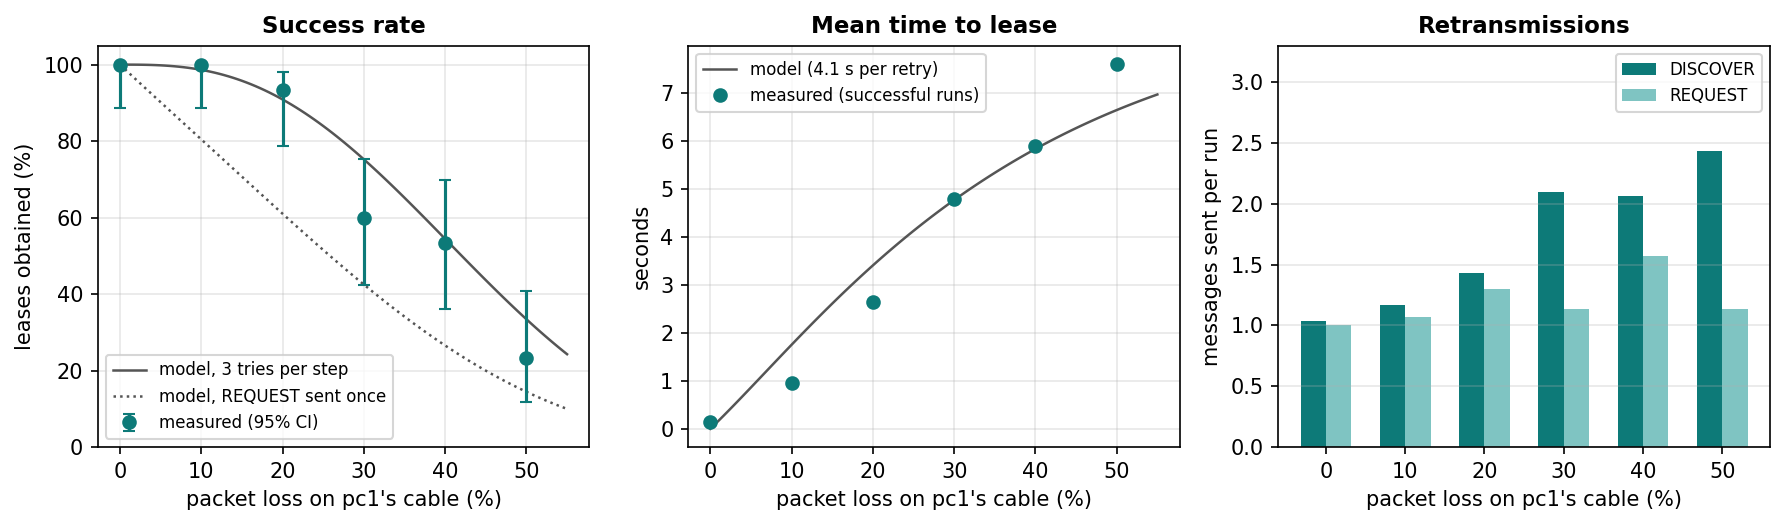
\includegraphics[width=\textwidth]{figures/dhcp_loss.png}
\caption{DHCP under packet loss: success rate, time to lease and retransmissions
(markers: measured; lines: model).}
\label{fig:loss}
\end{figure}

\section{Analysis}

\subsection{Correctness}
Every test passed. The ARP scenario reproduces each behaviour of RFC~826 that was
implemented, and all 13 DHCP functional tests produced the expected address, reply or
silence. Three results are worth noting. First, \textbf{interoperability}: BusyBox
\texttt{udhcpc}, written independently of this project, obtained a lease from our server
(F4), and \texttt{tcpdump}, an independent decoder, parses every field of our packets
correctly (C1). Both programs therefore follow the standard rather than merely agreeing
with each other. Second, the capture shows DISCOVER leaving with source address
\texttt{0.0.0.0}, as RFC~2131 requires for a client that has no address yet. Third, the
silent cases (F6--F9) matter as much as the replies. A server that answered a REQUEST
addressed to another server, or a stranger's INIT-REBOOT, would disrupt clients on a
network with several servers.

The \emph{bad udp cksum} warnings that \texttt{tcpdump -vv} prints for the captured DHCP
packets are an artifact of the capture, not an error. On veth interfaces Linux leaves the
UDP checksum to be filled in by ``hardware'' (checksum offload), and the capture point
sees the packet before that happens. The receiving sockets accept every packet.

\subsection{ARP Traffic and the Value of the Cache}
\label{sec:arpanalysis}
With $N$ hosts there are $N(N-1)$ ordered lookups per round. Yet round~1 needed only
\emph{half} as many requests, $N(N-1)/2$ (Table~\ref{tab:arptraffic}), and round~2 needed
none at all. The halving comes from the rule that the \emph{target} of a request caches
the requester. When host $i$ resolves host $j$, $j$ learns $i$ for free, so the later
lookup $j\to i$ is a cache hit. The zero in round~2 is the cache itself: within the
60\,s TTL every mapping is already known.

The right half of Figure~\ref{fig:arptraffic} shows why this matters. A request is
broadcast, so the hub must deliver $N-1$ copies of it, and every host on the LAN must
receive and inspect it. Round~1 therefore costs $\frac{N(N-1)}{2}(N-1) + \frac{N(N-1)}{2}$
frames, which grows as $N^3$ (224 frames for only 8 hosts). Without the target-caching
rule it would double, and without any cache it would be paid again on \emph{every}
packet. This is why broadcast domains are kept small and why ARP caches exist. The cost
of caching is staleness: an entry can be wrong for up to its TTL after a mapping changes,
which is what gratuitous ARP is for (A4).

\subsection{ARP Has No Security}
Test A5 shows the classic weakness. Host B accepted the fake host's gratuitous ARP and
now sends all traffic for 192.168.1.1 to MAC \texttt{02:00:00:00:00:99}. Nothing in ARP
authenticates the sender, so any host on the LAN can redirect another host's traffic to
itself. This is \emph{ARP spoofing}, the basis of man-in-the-middle attacks on LANs. Our
host detects the conflict only because the victim was \emph{itself} the owner of the
claimed address. A third host cannot tell a legitimate change (a failover, a replaced
NIC) from an attack. Real networks defend with static entries for critical hosts and
with switches that perform \emph{Dynamic ARP Inspection}, which checks ARP packets
against the address assignments learned by \emph{DHCP snooping}.

\subsection{DHCP Reliability: Model vs.\ Measurement}
\label{sec:lossanalysis}
Each DHCP step needs a message to reach the server \emph{and} the reply to come back.
With loss probability $p$ on pc1's cable in each direction, one attempt succeeds with
probability $q=(1-p)^2$. The client makes up to three attempts per step, so a step
succeeds with probability $1-(1-q)^3$. A lease needs both steps, so
\[
P_{\text{lease}} = \bigl(1-(1-q)^3\bigr)^2, \qquad q=(1-p)^2 .
\]
Each failed attempt costs one 4\,s wait. Given that a step succeeds at attempt $k\le3$,
which happens with probability proportional to $q(1-q)^{k-1}$, the expected delay of a
successful lease is
$2\sum_{k=1}^{3}4(k-1)\,q(1-q)^{k-1}\big/\sum_{k=1}^{3}q(1-q)^{k-1}$.

Table~\ref{tab:loss} and Figure~\ref{fig:loss} compare the model with the measurements.
The model predicts 100\%, 99\%, 91\%, 75\%, 55\% and 33\% success at 0--50\% loss, and
the measured rates (100\%, 100\%, 93\%, 60\%, 53\% and 23\%) agree with it. Five of the six model values lie inside the 95\% interval of the
measurement. The exception is 30\% loss, where the model (75.2\%) sits just on the upper
edge of the interval (75\%). That gap is 1.9 standard errors, which is consistent with
sampling variation when 30 runs are made at each of six levels. More runs per level would
narrow the intervals. The time to lease also behaves as designed.
It takes a few milliseconds when nothing is lost, and every lost message adds one 4.1\,s
wait, so successful runs take $\approx0$, 4.1, 8.2 or 12.3\,s (Table~\ref{tab:loss},
mean column). A run that fails in the DISCOVER step gives up after
$3\times4.1=12.3$\,s. The single retransmission at 0\% loss was the very first run: its
first DISCOVER was sent while the freshly created virtual link was still coming up, and
the retransmission recovered it 4\,s later.

Retransmission is what keeps DHCP usable on a lossy link. With one attempt per step, a
lease would succeed with probability only $q^2$, which is 41\% at 20\% loss. The earlier
version of our client retransmitted DISCOVER but not REQUEST (\S\ref{sec:fixes}), so it
would have succeeded only $(1-(1-q)^3)\,q$ of the time, 61\% at 20\% loss, against 91\%
for the fixed client. The ``no REQ retry'' column of Table~\ref{tab:loss} shows the full
comparison.

\subsection{Problems Found and Fixed During Development}
\label{sec:fixes}
The code was reviewed against the RFCs before the final tests. The defects below were
found and corrected, and each is now covered by a test above. The first one was also
reproduced on the old code: with the server dropping the first REQUEST, the old client
gave up while the fixed client obtained the lease on its second attempt.
\begin{itemize}[leftmargin=1.6em]
  \item \textbf{DHCPREQUEST was never retransmitted.} An earlier version resent DISCOVER
  but, after sending REQUEST, only waited. One lost REQUEST or ACK made the whole lease
  fail. Merging both steps into one \texttt{exchange()} function fixed it (test L1).
  \item \textbf{Gratuitous ARP had no effect.} Hosts only looked at requests whose
  \texttt{tpa} was their own address, so announcements were ignored. The RFC~826 merge
  rule fixed it (A4, A5).
  \item \textbf{Packets were lost in the hub.} The hub read up to 512 bytes and treated
  them as one packet, so two packets arriving together lost the second. Fixed with
  \texttt{recvAll()} (A7).
  \item \textbf{Byte order and forwarding.} The 16-bit ARP fields were stored in host
  (little-endian) order, and the hub forwarded replies by IP instead of by MAC. Both now
  match a real network.
\end{itemize}

\subsection{Known Limitations and Possible Improvements}
\begin{itemize}[leftmargin=1.6em]
  \item \textbf{The ARP LAN is simulated.} Frames travel over TCP on localhost, without an
  Ethernet header. The virtual LAN of the DHCP part shows the same protocol run by the
  Linux kernel over real (virtual) Ethernet. A raw-socket version of \texttt{host} could
  run on that LAN directly.
  \item \textbf{The hub trusts registration.} It learns MACs from \texttt{REG} rather than
  from frames (as a learning switch would), and does not prevent two hosts from claiming
  the same IP. This is deliberate, since that is what makes test A5 possible.
  \item \textbf{No pending-packet queue in ARP.} A failed \texttt{resolve} just reports
  failure; a real stack queues the IP packet and retries the request.
  \item \textbf{The DHCP client stops after the ACK.} It does not renew (at $T_1=50\%$ of
  the lease), rebind ($T_2=87.5\%$), release, or ARP-probe the new address and DECLINE it
  if it is in use. On a NAK it exits rather than restarting from DISCOVER. The server
  already handles RELEASE, DECLINE and renewals.
  \item \textbf{The client uses a UDP socket.} This is why \texttt{rp\_filter} must be
  disabled in the PC namespaces. A raw \texttt{AF\_PACKET} socket would remove the need.
  \item \textbf{Leases are kept in memory.} Restarting the server forgets every lease. A
  production server stores them on disk and probes an address (ICMP or ARP) before
  offering it.
\end{itemize}

\section{Comments}

\paragraph{Evaluation of the Project.} ARP and DHCP are the two protocols every networked
machine uses before it can send its first real packet, which is exactly why they are
normally invisible. Implementing both made each design decision concrete. Examples are
why the DHCP client must use the broadcast flag, why the REQUEST is broadcast even though
the server is known, why the target of an ARP request caches the requester, and why an
OFFER must expire. The virtual LAN was the most useful part of the project. It turned an
exchange that normally happens in a few milliseconds inside a router into something we
could watch step by step: addresses appearing on the PCs, the lease table filling, and
the kernel's ARP cache resolving the addresses our own server had handed out.

\paragraph{Difficulty and Learning Outcomes.} The packet formats themselves were
straightforward. The difficult parts were the ones the RFCs mention briefly. These
include framing a message protocol over a TCP stream, receiving a broadcast reply on a
machine that has no address yet (which led us to Linux's reverse-path filter), the silent
cases a server must respect, and making two threads share an ARP cache safely. Testing
taught as much as implementing. Each of the bugs listed in the Analysis passed a simple
manual demonstration and appeared only under a targeted test: a dropped packet, two
packets in one \texttt{send()}, a host with a duplicate address. Comparing the
packet-loss measurements against a simple probability model also gave confidence that
the retransmission logic behaves exactly as designed.

\paragraph{Suggested Improvements.} (1) Complete the DHCP client state machine (renew,
rebind, release, and DECLINE after an ARP probe), which would connect the two halves of
the project directly. (2) Port the ARP host to raw sockets so it can run on the virtual
LAN next to the kernel's implementation. (3) Add a DHCP relay agent in a second subnet to
show the \texttt{giaddr} field in use.

\end{document}
